\section{Socrata (Open Source)}
% Versione Open Source
Socrata � una piattaforma sviluppata dall'omonimia societ� con sede negli Stati Uniti d'America. Socrata � un servizio "Software as a service".
Dal 10 aprile 2013 � disponibile anche in una versione Community Edition rilasciata come Open Source al fine di promuovere uno standard intorno ai dati aperti e far crescere la comunit�.

Il Socrata Open Data Server e le componenti che lo compongono sono stati resi disponibili con licenza Apache. 
L�architettura del sistema pu� quindi essere suddivisa in una serie di componenti separate che la compongono come mostrato in figura \ref{fig:socrata-architecture}.

\begin{figure}[htbp]
   \centering
   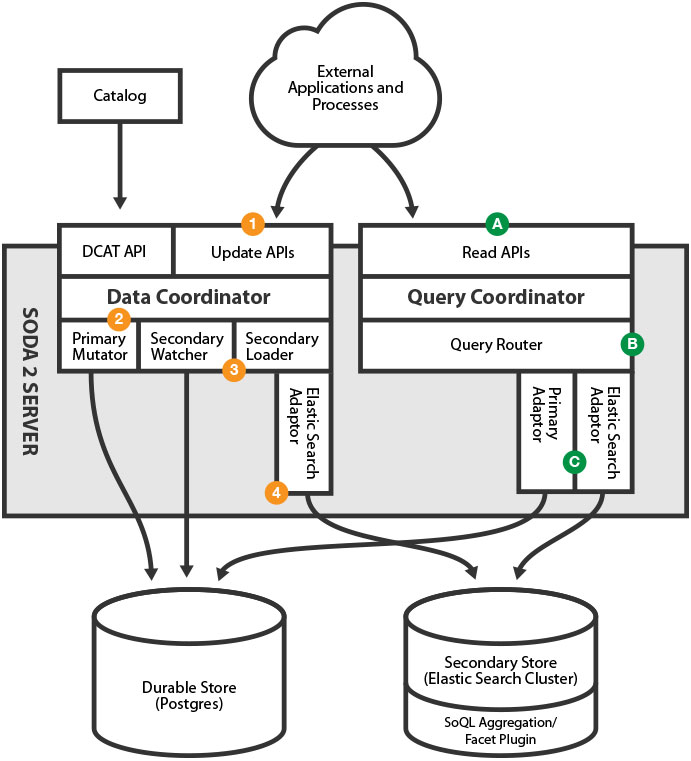
\includegraphics[scale=0.55]{img/socrata-architecture.jpg}
   \caption{Architettura di Socrata}
   \label{fig:socrata-architecture}
\end{figure}

SODA 2 fornisce quindi l�accesso ai dati puri attraverso SoQL (SODA Query Language) e delle semplici API per aggiornarli.
La scrittura avviene quindi attraverso un percorso che prevede il seguente percorso:
\begin{enumerate}
\item[\textcolor{Orange}{\ding{202}}] Un�applicazione o un processo inizia un�operazione sul SODA Server.
\item[\textcolor{Orange}{\ding{203}}] La richiesta viene trasformata in una serie di operazioni pi� elementari chiamante �mutations� e vengono passate al Data Coordinator in modo da essere eseguite sul database (Postgres).
\item[\textcolor{Orange}{\ding{204}}] Dopo che il Data Coordinator ha finito, il Secondary Watcher si sveglia e guarda se ci sono cambiamenti nel database che non sono ancora stati sincronizzati.
\item[\textcolor{Orange}{\ding{205}}] L�adattatore per l�archivio secondario (in questo caso Elastic Search) importa i dati dal primario.
Ci� permette in caso di guasti di re-sincronizzare il database.
\end{enumerate}

Mentre la lettura avviene attraverso:
\begin{enumerate}
\item[{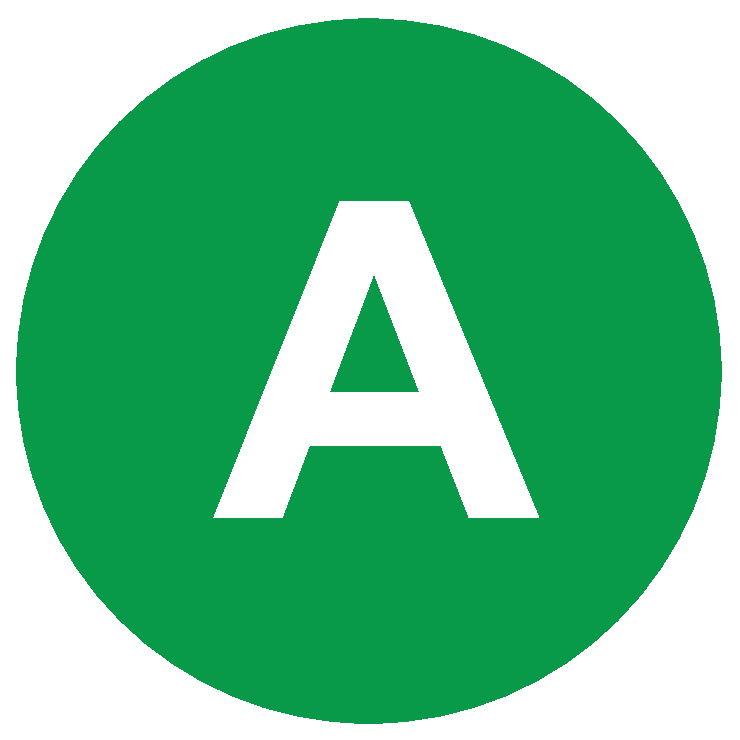
\includegraphics[scale=0.028]{img/A}}] Un�applicazione invia una richiesta al server SoQL. Questa viene analizzata come descritto serctitto in soql-reference.
\item[{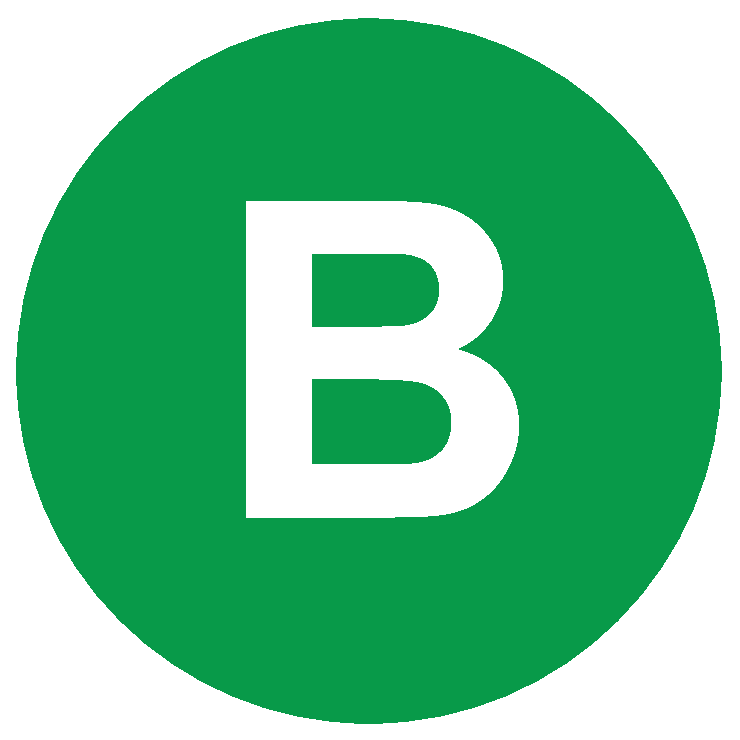
\includegraphics[scale=0.028]{img/B}}] Il Query Coordinator determina a quale database inviare la richiesta (in futuro ci portano essere diversi archivi secondari).
\item[{
\includegraphics[scale=0.028]{img/C}}] Il Query Coordinator passa fuori la query all�adattatore appropriato che esegue la query sull�archivio corretto e restituisce l'appropriato payload C-JSON.
\end{enumerate}

Ad oggi sono state rese disponibili con licenza Open Source solo alcune parti:

\begin{itemize}
\item \textbf{soql-reference}, Implementazione di riferimento del linguaggio di interrogazione SoQL.
\item \textbf{socrata-http}, Toolkit per la creazione di servizi HTTP.
\item \textbf{soql-es-adapter}, ElasticSearch Secondary Store per SoQL Data Service.
\item \textbf{socrata-csv}, Un sottile involucro Scalaish intorno ad opencsv.
\item \textbf{socrata-utils}, Classi-Utility utilizzate in tutto il Socrata Open Data Server.
\item \textbf{data-coordinator}, Coordina la distribuzione degli aggiornamenti tra archivi di dati primari e secondari.
\end{itemize}

La Community Edition condivide lo stesso core della versione proprietaria, ma al momento manca completamente il front-end per gestire comodamente i dataset che � invece presente nella versione SaaS.
Secondo la Roadmap intorno all'Agosto 2013 era previsto il rilascio della versione beta finale, compresa della documentazione e degli strumenti che avrebbero permesso di installare e rendere funzionate l'intero Open Data Server.

Socrata offre sia numerose API per gestire i dataset, che strumenti di visualizzazione che mostrano i dati caricati attraverso un sistema di preview tabellare dotato di filtri avanzati, oppure su diverse tipologie di mappe in caso di dati geolocalizzati.
Permette inoltre di esportare i dati in vari formati (CSV, XLS, XLSX, XML, JSON).

In Italia Socrata � stata usata con successo dalla Regione Lombardia con un centinaio di dataset pubblicati.